%Shortest path problem
\section{Shortest path problem}\label{shortestPathProblem}
	For route planning, routes through a network must be optimized in regards to one or even many criteria.
	A common criteria is the \textit{travel time}. Others include cost, number of transfers or restrictions
	in transportation types.
	
	In this chapter, we will first give an informal description of the \earliestArrivalProblem. Followed by
	the \shortestPathProblem, which is equivalent to the \earliestArrivalProblem for our graph-based network
	representations.
	
	Then, we introduce algorithms for solving the problem. First, for time-independent networks, then for time-dependent.
	Afterwards, we explain two solutions for combined networks, using multiple transportation modes. There, the problem
	description slightly changes by adding transportation mode restrictions.\\\\
	\begin{mydef}
		The earliest arrival problem asks for finding a \textnormal{route} in a network with following properties
		\begin{itemize}
			\item[1.] The route must start at $s$ and end at $t$.
			\item[2.] The departure time at $s$ is $\tau$.
			\item[3.] All other applicable routes must have a greater travel time, i.e. arrive later at $t$.
		\end{itemize}
		Points $s$ and $t$ are given source and target points in the network respectively. $\tau$ is the desired departure time,
		it may be ignored for a time-independent network.
	\end{mydef}
	\begin{mydef}
		Given a graph $G = (V, E)$, source and target nodes $s, t \in V$ and a desired departure time $\tau$, the shortest path
		problem asks for a path $p$ (see \defref{path}) which
		\begin{itemize}
			\item[1.] begins at $s$ and ends at $t$,
			\item[2.] has the smallest weight of all applicable paths.
		\end{itemize}
		The arrival time at $t$ is $\tau$ plus the weight of $p$. In a time-dependent
		graph $\tau$ must be used to ensure correct edge weights. The path $p$ is called \textnormal{shortest path}.
	\end{mydef}\quad\\
	Additionally, we consider a special variant of the shortest path problem:
	\begin{mydef}
		The many-to-one shortest path problem is a variation of the shortest path problem
		where the source consists of a set of source nodes $S \subseteq V$.

		The problem asks for the path $p$ that starts at the source $s \in S$ which minimizes the path weight.
	\end{mydef}

%Time-independent
\subsection{Time-independent}
	Route planning in time-independent networks is a very well studied problem.
	Many efficient solutions to the shortest path problem exists. We introduce a very basic algorithm, \dijkstra
	and a simple improvement based on heuristics, \astar.
	% Time-independent example
	\begin{figure}[!ht]
		 \begin{center}
			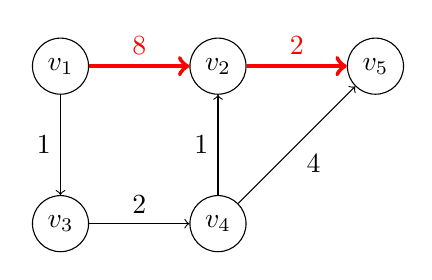
\begin{tikzpicture}[y = -1cm]
			 	% Nodes
			 	\node[circle, draw] (v1) at (0, 0) {$v_1$};
			 	\node[circle, draw] (v2) at (2, 0) {$v_2$};
			 	\node[circle, draw] (v3) at (0, 2) {$v_3$};
			 	\node[circle, draw] (v4) at (2, 2) {$v_4$};
			 	\node[circle, draw] (v5) at (4, 0) {$v_5$};
			 	
			 	% Edges
			 	\draw[ultra thick, ->, color = red] (v1) to node[above] {$8$} (v2);
			 	\draw[ultra thick, ->, color = red] (v2) to node[above] {$2$} (v5);
			 	\draw[->] (v1) to node[left] {$1$} (v3);
			 	\draw[->] (v3) to node[above] {$2$} (v4);
			 	\draw[->] (v4) to node[left] {$1$} (v2);
			 	\draw[->] (v4) to node[below right] {$4$} (v5);
			\end{tikzpicture}\qquad\qquad\qquad
			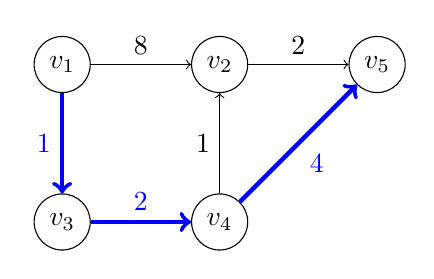
\begin{tikzpicture}[y = -1cm]
			 	% Nodes
			 	\node[circle, draw] (v1) at (0, 0) {$v_1$};
			 	\node[circle, draw] (v2) at (2, 0) {$v_2$};
			 	\node[circle, draw] (v3) at (0, 2) {$v_3$};
			 	\node[circle, draw] (v4) at (2, 2) {$v_4$};
			 	\node[circle, draw] (v5) at (4, 0) {$v_5$};
			 	
			 	% Edges
			 	\draw[->] (v1) to node[above] {$8$} (v2);
			 	\draw[->] (v2) to node[above] {$2$} (v5);
			 	\draw[ultra thick, ->, color = blue] (v1) to node[left] {$1$} (v3);
			 	\draw[ultra thick, ->, color = blue] (v3) to node[above] {$2$} (v4);
			 	\draw[->] (v4) to node[left] {$1$} (v2);
			 	\draw[ultra thick, ->, color = blue] (v4) to node[below right] {$4$} (v5);
			\end{tikzpicture}\quad\\\phantom{v}\quad\\
			\begin{tikzpicture}[y = -1cm]
			 	% Nodes
			 	\node[circle, draw] (v1) at (0, 0) {$v_1$};
			 	\node[circle, draw] (v2) at (2, 0) {$v_2$};
			 	\node[circle, draw] (v3) at (0, 2) {$v_3$};
			 	\node[circle, draw] (v4) at (2, 2) {$v_4$};
			 	\node[circle, draw] (v5) at (4, 0) {$v_5$};
			 	
			 	% Edges
			 	\draw[->] (v1) to node[above] {$8$} (v2);
			 	\draw[ultra thick, ->, color = darkgreen] (v2) to node[above] {$2$} (v5);
			 	\draw[ultra thick, ->, color = darkgreen] (v1) to node[left] {$1$} (v3);
			 	\draw[ultra thick, ->, color = darkgreen] (v3) to node[above] {$2$} (v4);
			 	\draw[ultra thick, ->, color = darkgreen] (v4) to node[left] {$1$} (v2);
			 	\draw[->] (v4) to node[below right] {$4$} (v5);
			\end{tikzpicture}
		\end{center}
		\caption{Example for a time independent network, represented by a road graph.
		The figure shows three paths from $v_1$ to $v_5$. From top left to bottom right, the path
		weights are $10$, $7$ and $6$. The last example represents the shortest path from $v_1$ to $v_5$.}
		\label{timeIndependentExample}
	\end{figure}\quad\\
	The network shown by \figref{timeIndependentExample} acts as toy example for this section.

%Dijkstra
\subsubsection{Dijkstra}
	\dijkstra \libref{dijkstra} is a simple approach to solving the shortest path problem. It can be viewed
	as the logical extension of breadth-first search (\bfs) \libref{dijkstra} in weighted graphs. The algorithm
	revolves around a priority queue where it stores neighboring nodes, sorted by their shortest path cost.
	In each round, the node with the smallest shortest path cost is \textit{relaxed}. That is, all its neighboring,
	not already relaxed, nodes are added to the queue. The algorithm terminates as soon as the target node has been relaxed.
	\algoref{dijkstra} gives a formal description.
	% Dijkstra implementation
	\IncMargin{1em}
	\begin{algorithm}
		\SetKwInOut{Input}{input}
  		\SetKwInOut{Output}{output}
  		\SetKw{Break}{break}
  		\SetKwData{undef}{undefined}\SetKwData{currentDist}{currentDist}
		\SetKwFunction{dist}{dist}\SetKwFunction{prev}{prev}
		\BlankLine
		\Input{graph $G = (V, E)$, source $s \in V$, target $t \in V$}
		\Output{shortest path from $s$ to $t$}
		\BlankLine
		\tcp{Initialization}
		\For{$v \in V$}{
			$\dist(v) \leftarrow \infty$\;
			$\prev(v) \leftarrow \undef$\;
		}
		\BlankLine
		$\dist(s) \leftarrow 0$\;
		$Q \leftarrow \{s\}$\;
		\BlankLine
		\tcp{Compute shortest paths}
		\While{$Q$ is not empty}{
			$u \leftarrow \argmin_{u' \in Q} \dist(u')$\;
			$Q \leftarrow Q \setminus \{u\}$\;
			\BlankLine
			\If{$u == t$}{
				\Break\;
			}
			\BlankLine
			\tcp{Relax $u$}
			\For{outgoing edge $(u, w, v) \in E$}{
				$\currentDist \leftarrow \dist(u) + w$\;
				\If{$\currentDist < \dist(v)$}{
					\tcp{Improve distance by using this edge}
					$\dist(v) \leftarrow \currentDist$\;
					$\prev(v) \leftarrow u$\;
					$Q \leftarrow Q \cup \{v\}$\;
				}
			}
		}
		\BlankLine
		\tcp{Extract path by backtracking}
		$p \leftarrow$ empty path\;
		$u \leftarrow t$\;
		\While{$\prev(u) \neq \undef$}{
			$w \leftarrow \dist(u) - \dist(\prev(u))$\;
			prepend $(\prev(u), w, u)$ to $p$\;
			$u \leftarrow \prev(u)$\;
		}
		prepend $s$ to $p$\;
		\Return $p$\;
		\BlankLine
		\caption{Dijkstra's algorithm for computing shortest paths in time-independent graphs.}\label{dijkstra}
	\end{algorithm}\DecMargin{1em}\quad\\\\
	To familiarize with the algorithm, we step through the execution for the graph shown by \figref{timeIndependentExample},
	with $v_1$ as source and $v_5$ as target node.
	
	The $\dist$ function, often implemented as array, stores the tentative shortest path weight to the given node.
	$\prev$ is used for path extraction at the end, it stores the parent nodes used for the shortest paths represented by $\dist$.
	The algorithm starts by initializing both collections with default values. Initially the distance to all nodes, except the source, is unknown.
	Thus, $\infty$ is used for them. $Q$ represents the list of nodes that need to be processed, usually implemented as priority queue.
	Initially, it only holds the source node $s$.
	
	In the example $Q$ is initially $\{v_1\}$. The algorithm then relaxes $v_1$ and stores distances to its neighbors:
	\begin{center}
		\begin{tabular}{CC}
			\dist(v_2) = 8	&\prev(v_2) = v_1,\\
			\dist(v_3) = 1	&\prev(v_3) = v_1
		\end{tabular}
	\end{center}
	Additionally, the queue $Q$ is updated, it is
	\begin{align*}
		Q	&= \{v_2, v_3\}.
	\end{align*}
	The next iteration of the loop starts and the node with the smallest distance is chosen, i.e. $v_3$. The node is relaxed and we receive
	\begin{center}
		\begin{tabular}{CC}
			\dist(v_4) = 3	&\prev(v_4) = v_3,\\
			\multicolumn{2}{c}{$Q = \{v_2, v_4\}.$}
		\end{tabular}
	\end{center}
	The next node is $v_4$, yielding
	\begin{center}
		\begin{tabular}{CC}
			\dist(v_2) = 4	&\prev(v_2) = v_4,\\
			\dist(v_5) = 7	&\prev(v_5) = v_4,\\
			\multicolumn{2}{c}{$Q = \{v_2, v_5\}.$}
		\end{tabular}
	\end{center}
	Note that $v_4$ improves the distance to $v_2$. The previous values for $v_2$ are overwritten and the
	tentative shortest path to $v_2$ uses $(v_4, 1, v_2)$ and not $(v_1, 8, v_2)$ anymore.
	In the next round $v_2$ is relaxed which improves the distance to $v_5$:
	\begin{center}
		\begin{tabular}{CC}
			\dist(v_5) = 6	&\prev(v_5) = v_2,\\
			\multicolumn{2}{c}{$Q = \{v_5\}.$}
		\end{tabular}
	\end{center}
	The only node left is the target node $v_5$ now. It is relaxed and the loop terminates.
	The algorithm backtracks the parent pointer
	\begin{align*}
		\prev(v_5)	&= v_2,\\
		\prev(v_2)	&= v_4,\\
		\prev(v_4)	&= v_3,\\
		\prev(v_3)	&= v_1,\\
		\prev(v_1)	&= \vundef
	\end{align*}
	and constructs the shortest path
	\begin{align*}
		p	&= (v_1, 1, v_3)(v_3, 2, v_4)(v_4, 1, v_2)(v_2, 2, v_5)
	\end{align*}
	which is the path shown by the last example in the figure.

%A*
\subsubsection{\astar and \alt}\label{alt}
	An important observation of \dijkstra is that, if it settles the shortest path distance to a node, then,
	all nodes which are closer to the source, were already settled in a previous round.
	
	Moreover, the algorithm explores the graph in all directions equally. It has no sense of \textit{goal direction}.\\\\
	The \astar algorithm \libref{alt} is a simple extension of \dijkstra which improves its efficiency by steering the
	exploration more towards the target. \figref{dijkstra_vs_astar} illustrates this by comparing the \textit{search space}
	of both algorithms. The search space of \astar is smaller and much more directed to the target node $t$.
	% A-star vs Dijkstra
	\begin{figure}[!ht]
		 \begin{center}
			\includegraphics[scale=0.5]{res/dijkstra_vs_astar}
		\end{center}
		\caption{Schematic illustration of a query processed by \dijkstra (left) and \astar (right).
			The highlighted areas indicate the \textit{search space}, i.e. the nodes the algorithm has explored already.
			The illustration is from \libref{routePlanningOverview}.}
		\label{dijkstra_vs_astar}
	\end{figure}\quad\\
	Unfortunately, computing the exact goal direction is as hard as computing the shortest path to the target.
	Therefore, a heuristic is used to approximate the direction. The choice of the heuristic heavily depends on the underlying network.
	In the worst case, a heuristic may not improve over \dijkstra and the same search space is received. In the best case,
	the algorithm explores only the nodes on the shortest path.
	
	Such a heuristic must fulfill two properties, formulated by \defref{heuristic}.
	\begin{mydef}\label{heuristic}
		Given a graph $G = (V, E)$, a metric $\dist$ on $V$ (see \defref{metric}),
		a \textnormal{heuristic} is a function $h: V \times V \to \mathbb{R}_{\ge 0}$ which approximates $\dist$.
		The heurstic $h$ must be
		\begin{itemize}
			\item[1.] \textnormal{admissable}, i.e. never overestimate:
				\begin{align*}
					\forall u, t \in V: h(u, t) \le \dist(u, t)
				\end{align*}
			\item[2.] \textnormal{monotone}, i.e. satisfy the triangle inequality:
				\begin{align*}
					\forall t \in V\,\forall (u, w, v) \in E: h(u, t) \le w + h(v, t)
				\end{align*}
		\end{itemize}
	\end{mydef}\quad\\
	Given such a heuristic $h$, the \astar algorithm is received by adjusting \textbf{line 7} of \algoref{dijkstra} to
	\begin{align*}
		u \leftarrow \argmin_{u' \in Q} \dist(u') + h(u', t).
	\end{align*}
	This will prefer nodes that are estimated to be closer to the target before others. By that, the algorithms search space
	first expands into a direction that minimizes the distance according to the heuristic $h$.\\\\
	A common choice for a simple heuristic is the \textit{as-the-crow-flies} metric (see \defref{asTheCrowFlies}).
	The properties are easily verified. A theoretically shortest path has the shortest possible distance and uses
	the fastest available transportation mode. This is exactly the path represented by the \textit{straight-line} distance,
	computed by the \textit{as-the-crow-flies} metric. It can thus never overestimate. It is also trivially monotone since it is a metric,
	i.e. the triangle inequality holds for all elements.
	
	A heuristic is a good choice if it approximates the actual shortest path distance well. As such, the \textit{as-the-crow-flies} heuristic works well
	on networks with a high connectivity in all directions. For example a residential area of a city without one way streets. Unfortunately, in road
	networks, the common case is to first drive into the opposite direction in order to reach a fast highway. This even gets worse on networks
	where the importance of nodes heavily differ, such as public transit networks. For train networks, the typical case is that one first needs
	to travel to a main station. This is obviously due to a main station having a much better connectivity and faster trains available.
	Because of that, the effectiveness of \textit{as-the-crow-flies} is very limited on such networks.\\\\
	The \textit{landmark heurstic} partially solves the issue. An \astar algorithm using the landmark heuristic is called \alt \libref{alt},
	which stands for \textit{landmarks and triangle inequality}.
	
	The heuristic provides a more generic approach by approximating the distance
	between nodes $u$ and $v$ by using pre-computed distances with pre-determined nodes $l$, called \textit{landmarks}.
	\begin{mydef}
		Given a set of landmarks $L \subseteq V$, the heuristic $\landmarks$ is defined by
		\begin{align*}
			\landmarks(u, v)	&= \max_{l \in L} \left(\max \{\dist(u, l) - \dist(v, l), \dist(l, v) - \dist(l, u)\}\right).
		\end{align*}
	\end{mydef}\quad\\
	Obviously, the heuristic improves if the set of landmarks is increased. However, actual shortest path distances from all landmarks
	to all other nodes in the graph must be pre-computed. With an increasing amount of landmarks the pre-computation might not
	be feasible anymore because it takes too long or consumes too much space. Note that if $L = V$, the heuristic becomes the
	actual shortest path distance function, i.e. $\landmarks = \dist$.
	
	In practice, an amount between $20$ and $50$ randomly chosen nodes seems to be a good compromise.
	Refer to \libref{alt} for a detailed analysis.\\\\
	The computation of the actual shortest path distances, to and from the landmarks, can be done by using \dijkstra. But, instead of
	running the algorithm for all pairs of nodes, the distances can be obtained with two runs only. Therefore, the algorithm is slightly modified by dropping
	\textbf{lines 9} and \textbf{10}, such that the algorithm relaxes the whole network. By that, a single run of \dijkstra with a landmark $l$ as source,
	computes the distances $\dist(l, v)$ to all nodes $v$ in the network. By reversing the graph, i.e. edges $(u, w, v)$ become $(v, w, u)$, the distances to
	the landmarks can be obtained analogously with $l$ as source again. Depending on the graph implementation, reversal can be done
	in $\mathcal{O}(1)$ by only implicitly reversing the edges.

%Time-dependent
\subsection{Time-dependent}
	Approaches designed for time-independent networks, such as \alt, have an important drawback. Optimization is always done on
	assuming that edge costs are constant. However, in a time-dependent network, this is not the case. The weight of an edge is
	dependent on the departure time, which is not known in advance.\\\\
	\dijkstra and its variants \astar and \alt can easily be adapted to also work in time-dependent networks by taking the departure
	time into consideration when computing the weight of an edge. However, their effectiveness is very limited.
	Nonetheless, they where used for a long time for time-dependent networks too. With increasing research on route
	planning in time-dependent networks, more effective algorithms, such as \transferPatterns \libref{transferPatterns}
	and \csa \libref{csa}, were developed. Many of them do not use graphs and prefer data-structures that are designed
	for time-dependent data, such as \textit{timetables} (see \sectionref{timetable_sec}).

%Connection scan
\subsubsection{Connection scan}\label{csa}
	Connection scan (\csa) \libref{csa} is an algorithm for route planning specially designed for time-dependent networks,
	such as public transit networks. It processes the network represented as timetable, as defined by \defref{timetable}.\\\\
	The algorithm is very simple. All connections of the timetable are sorted by their departure time.
	Give a query connections are explored increasing in their departure time. The algorithm is fast primarily due to the fact that
	connections can be maintained in a simple array. In contrast to \dijkstra, it does not need to maintain a priority queue or
	other more complex data-structures. Arrays are heavily optimized and benefit from a lot of effects, like cache locality \libref{cacheLocality}.
	% CSA implementation
	\IncMargin{1em}
	\begin{algorithm}
		\SetKwInOut{Input}{input}
  		\SetKwInOut{Output}{output}
  		\SetKw{Break}{break}
  		\SetKwData{undef}{undefined}
		\BlankLine
		\Input{timetable $(S, T, C, F)$, source $s \in S$, target $t \in S$, departure time $\tau$}
		\Output{shortest path from $s$ to $t$}
		\BlankLine
		\tcp{Initialization}
		\lFor{$u \in S$}{
			$S[u] \leftarrow \infty$
		}
		\lFor{$o \in T$}{
			$T[o] \leftarrow \undef$
		}
		\lFor{$u \in S$}{
			$J[u] \leftarrow (\undef, \undef, \undef)$
		}
		\BlankLine
		\For{$f = (u_{\dep}, d, u_{\arr}) \in F : u_{\dep} = s$}{
			$S[u_{\arr}] \leftarrow \tau + d$\;
			$J[u_{\arr}] \leftarrow (\undef, \undef, f)$\;
		}
		\BlankLine
		\tcp{Explore connections increasing in departure time}
		$c_0 \leftarrow \argmin_{(u_{\dep}, u_{\arr}, \tau_{\dep}, \tau_{\arr}, o) \in C : \tau_{\dep} \ge \tau} \tau_{\dep}$\;
		\For{$c = (u_{\dep}, u_{\arr}, \tau_{\dep}, \tau_{\arr}, o) \in C$ increasing by $\tau_{\dep}$, starting from $c_0$}{
			\If{$\tau_{\dep} \ge S[t]$}{
				\Break\;
			}
			\BlankLine
			\If{$T[o] \neq \undef \lor \tau_{\dep} \ge S[u_{\dep}]$}{
				$T[o] \leftarrow c$\;
				\If{$\tau_{\arr} < S[u_{\arr}]$}{
					\For{$f = (v_{\dep}, d, v_{\arr}) \in F : v_{\dep} = u_{\arr}$}{
						\If{$\tau_{\arr} + d < S[v_{\arr}]$}{
							$S[v_{\arr}] \leftarrow \tau_{\arr} + d$\;
							$J[v_{\arr}] \leftarrow (T[o], c, f)$\;
						}
					}
				}
			}
		}
		\BlankLine
		\tcp{Extract path by backtracking}
		$p \leftarrow$ empty path\;
		$u \leftarrow t$\;
		\While{$c_{\enter} \neq \undef : (c_{\enter}, c_{\exit}, f) = J[u]$}{
			prepend $f$ to $p$\;
			prepend the part of the trip between $c_{\enter}$ and $c_{\exit}$ to $p$\;
			$u \leftarrow v_{\dep} : (v_{\dep}, v_{\arr}, \tau'_{\dep}, \tau'_{\arr}, o) = c_{\enter}$\;
		}
		prepend $f : (\undef, \undef, f) = J[s]$ to $p$\;
		\Return $p$\;
		\BlankLine
		\caption{Connection scan algorithm for computing shortest paths in time-dependent networks, represented by timetables.}\label{csa_algo}
	\end{algorithm}\DecMargin{1em}\quad\\\\
	\algoref{csa_algo} shows the full connection scan algorithm. \todo{Explain the algorithm, make an example...}

%Multi-modal
\subsection{Multi-modal}
	Blabla

%Modified Dijkstra
\subsubsection{Modified Dijkstra}\label{modifiedDijkstra}
	Blabla

%Access nodes
\subsubsection{Access nodes}\label{accessNodes}
	Blabla

%Other algorithms
\subsection{Other algorithms}
	Blabla